\documentclass[11pt, t]{beamer} 
\setcounter{MaxMatrixCols}{20}
\usepackage{multimedia}
\usepackage{hyperref} 

%--------------------------------------------------------------------------------------------------
% Set language options and load DSS beamer template
%    Set the directory of the template by \newcommand{\StyleDir}{<yourDir>}. <yourDir> can be a
%    relative or absolute path and is necessary to find the images contained in the template.
%--------------------------------------------------------------------------------------------------
\newcommand{\SlideName}{Slide}
%\newcommand{\StyleDir}{E:/dss_tools/latex/dss_beamer_template/style/}
\newcommand{\StyleDir}{style/}

\input{\StyleDir dss_beamer}
%\input{\StyleDir dss_beamer_squeeze}


%--------------------------------------------------------------------------------------------------
% Pack four slides on one DIN A4 page
%--------------------------------------------------------------------------------------------------
%\makeHandout


%--------------------------------------------------------------------------------------------------
% Title settings, e.g. author, title, ... 
%--------------------------------------------------------------------------------------------------
\title[Speech Recognition - EQ 2340]{Speech Recognition - EQ2340}
\subtitle{HMM (Hidden Markov Models)}
\author[Alessio Russo and Lars Lindemann]{Alessio Russo  	Lars Lindemann  }
\date[2015/11/03]{3rd November, 2015}
\institute[KTH]{Royal Institute of Technology (KTH, Stockholm)  \vspace{1mm}}

%--------------------------------------------------------------------------------------------------
% Start of document
%--------------------------------------------------------------------------------------------------
\begin{document}

\setbeamercovered{dynamic}
\frame[plain]{\titlepage      % titlepage without headline, footline and frametitle
\setcounter{framenumber}{0}}  % reset pagenumber (firstpage will be No. 1)

%--------------------------------------------------------------------------------------------------
% Table of contents
%--------------------------------------------------------------------------------------------------
\section*{Content}
% --- Give this slide the name 'contentframe' so it can be repeated later later on
\begin{frame}<1>[label = contentframe]{Content}{\quad} 
	\setcounter{tocdepth}{2}
  \tableofcontents  
\end{frame}

%--------------------------------------------------------------------------------------------------
% Include sections
%--------------------------------------------------------------------------------------------------
%--------------------------------------------------------------------------------------------------
% Präsentation ICC-System:
%		Stand der Dinge in Sachen Rückkopplungskompensation und Ausblick
%
%--------------------------------------------------------------------------------------------------


\section{Introduction}

%~~~~~~~~~~~~~~~~~~~~~~~~~~~~~~~~~~~~~~~~~~~~~~~~~~~~~~~~~~~~~~~~~~~~~~~~~~~~~~~~~~~~~~~~~~~~~~~~~~
% New subsection
%~~~~~~~~~~~~~~~~~~~~~~~~~~~~~~~~~~~~~~~~~~~~~~~~~~~~~~~~~~~~~~~~~~~~~~~~~~~~~~~~~~~~~~~~~~~~~~~~~~
\subsection{Problem Formulation}

%--------------------------------------------------------------------------------------------------
% New frame
%--------------------------------------------------------------------------------------------------
\begin{frame}{\insertsection}{\insertsubsection}   
 
\medskip
\headline{Speech Recognition of a limited speech corpus}\\
\only<2-3>{
\begin{itemize}
\item High demand in industry
\item Usage in current systems (e.g. Siri)
\item Easy to understand general principle
\end{itemize}
}
\only<3>{
\headline{Speech Corpus}
\begin{itemize}
\item General speech corpus to form sentences
\item Multisyllabic, similar and short words to challenge the system
\end{itemize}
}
\only<4>{
\vspace{0mm}
\begin{center}
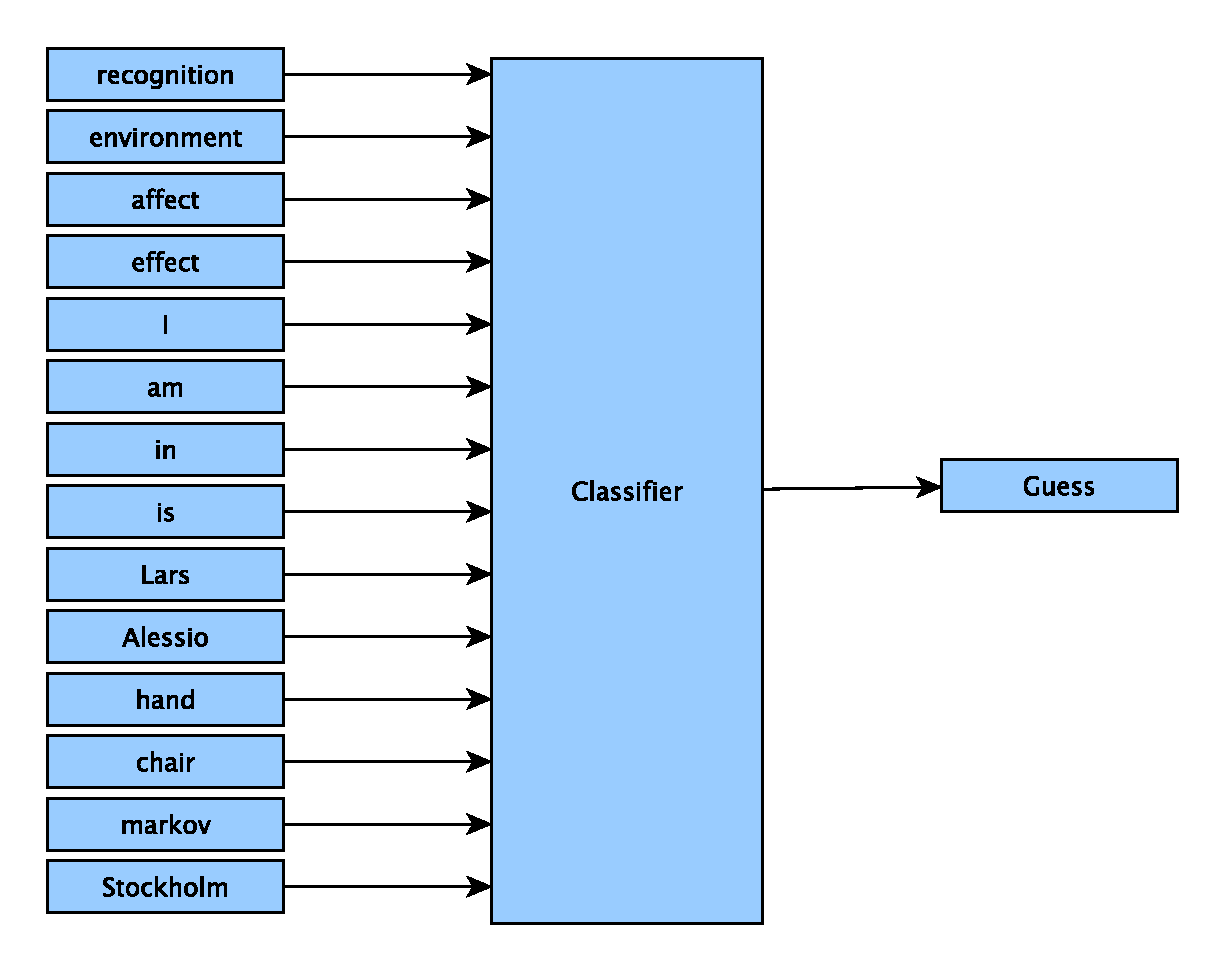
\includegraphics[width=0.65\textwidth]{figures/problem}
\end{center}}
\only<5>{
\begin{itemize}
\item Two examples...
\end{itemize}
\movie[externalviewer]{Lars: affect}{lars_affect-01.wav}\\
\movie[externalviewer]{Natalie: recognition}{natalie_recognition-11.wav}
}
%talk about application and data
%why did we choose this project
\end{frame}
 
 
 
 
 %~~~~~~~~~~~~~~~~~~~~~~~~~~~~~~~~~~~~~~~~~~~~~~~~~~~~~~~~~~~~~~~~~~~~~~~~~~~~~~~~~~~~~~~~~~~~~~~~~~
% New subsection
%~~~~~~~~~~~~~~~~~~~~~~~~~~~~~~~~~~~~~~~~~~~~~~~~~~~~~~~~~~~~~~~~~~~~~~~~~~~~~~~~~~~~~~~~~~~~~~~~~~
\subsection{System architecture}

%--------------------------------------------------------------------------------------------------
% New frame
%--------------------------------------------------------------------------------------------------
\begin{frame}{\insertsection}{\insertsubsection}   
 
\headline{Overview of the Implementation}
\vspace{0mm}
\begin{center}
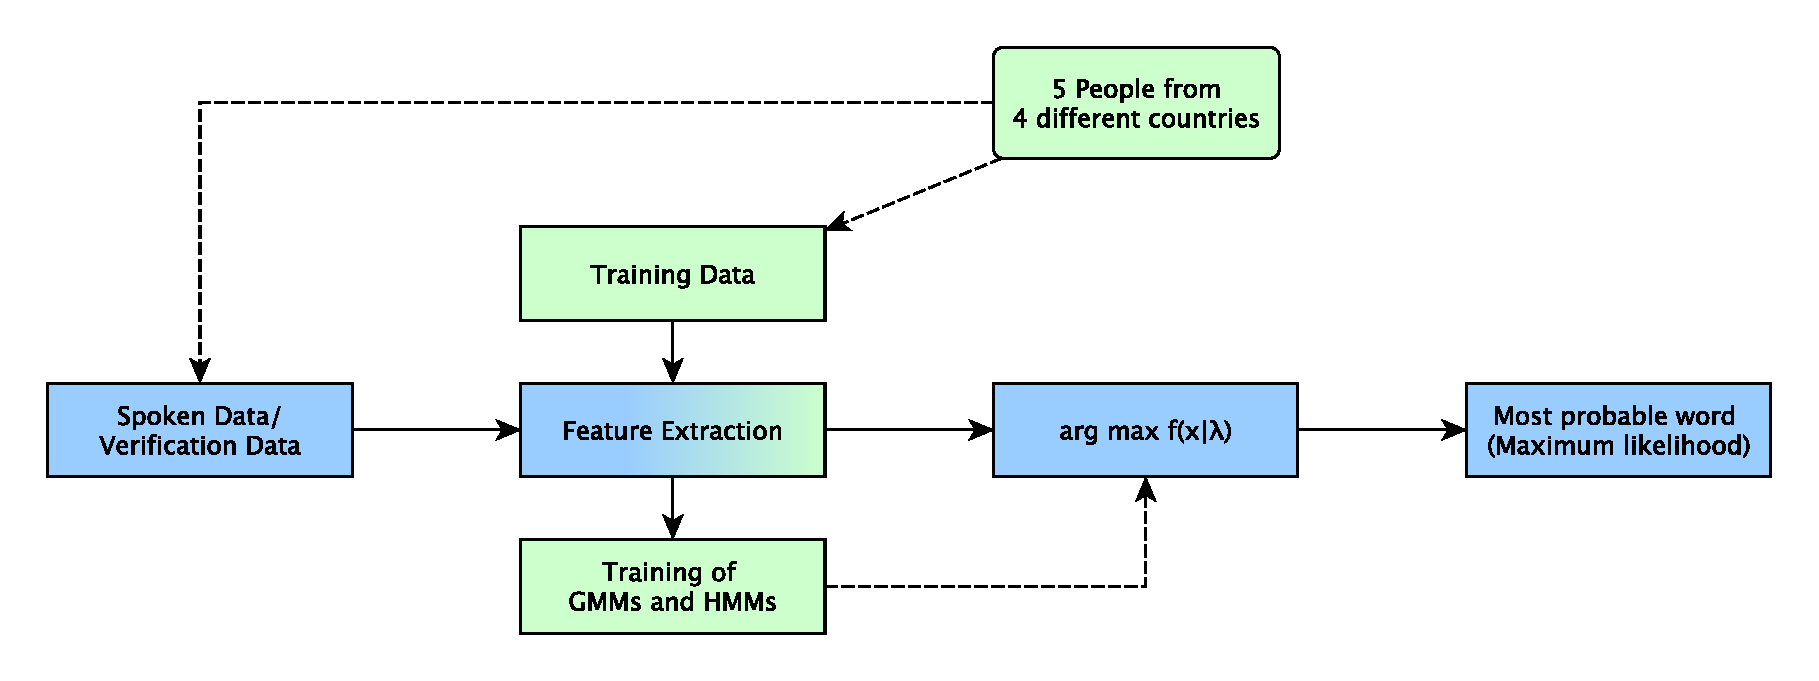
\includegraphics[width=0.85\textwidth]{figures/system}
\end{center}
%picture and rough description of the system
\only<2>{
\begin{itemize}
\item Distinguish between training and validation/live demonstration
\end{itemize}}
 \end{frame}
 
 

 
\againframe<2>{contentframe}   % repeat the table of contents
%--------------------------------------------------------------------------------------------------
% Präsentation ICC-System:
%		Stand der Dinge in Sachen Rückkopplungskompensation und Ausblick
%
%--------------------------------------------------------------------------------------------------


\section{System Design, Training and Testing}

%~~~~~~~~~~~~~~~~~~~~~~~~~~~~~~~~~~~~~~~~~~~~~~~~~~~~~~~~~~~~~~~~~~~~~~~~~~~~~~~~~~~~~~~~~~~~~~~~~~
% New subsection
%~~~~~~~~~~~~~~~~~~~~~~~~~~~~~~~~~~~~~~~~~~~~~~~~~~~~~~~~~~~~~~~~~~~~~~~~~~~~~~~~~~~~~~~~~~~~~~~~~~
\subsection{Feature Extraction}

%--------------------------------------------------------------------------------------------------
% New frame
%--------------------------------------------------------------------------------------------------
\begin{frame}{\insertsection}{\insertsubsection}   
 \headline{Possible problems}
\begin{itemize}
\uncover<1->{
\item Pitch}
\uncover<2->{
\item Different speakers (absolut output value)}
\uncover<3->{
\item Noise}
\end{itemize}

\only<4->{
\headline{Continuous feature vectors}
\medskip
\begin{itemize}
\uncover<4->{
\item 13 MFCC (Mel-frequency cepstrum coefficients)}
\uncover<5->{
\item 26 dynamical features (independent of absolute value)}
\uncover<6->{
\item 30 ms time frame}
\end{itemize}}




 \end{frame}
 
  \subsection{HMM}
 %--------------------------------------------------------------------------------------------------
% New frame
%--------------------------------------------------------------------------------------------------
\begin{frame}{\insertsection}{\insertsubsection}   
 \medskip
\headline{Number of States for left-right HMM}
\begin{itemize}
\uncover<1->{
\item Trade off: too few parameters vs. amount of training data}
\uncover<2->{
\item Also: Limited training data}
\uncover<3->{
\item State assignment due to syllables + start/end state}

\end{itemize}
\vspace{5mm}
\only<4->{
\begin{columns}
\column{0.4\textwidth}
\textit{environmnent}: 6 states
\column{0.5\textwidth}
\textit{chair}: 4 states
\end{columns}}
\vspace{5mm}
\only<5->{
\headline{Output distributions}
\begin{itemize}
\item GMM (Gaussian Mixture Models)
\end{itemize}}




 
 \end{frame}
 
\subsection{Training data and validation set}
 %--------------------------------------------------------------------------------------------------
% New frame
%--------------------------------------------------------------------------------------------------
\begin{frame}{\insertsection}{\insertsubsection}   
 \headline{Recorded data}
 \begin{itemize}
 \uncover<1->{
 \item 5 people: 15 recordings per word
 \item One person has been disregarded
 \item 840 recordings in total, 60 per word}
 \end{itemize}
 \vspace{8mm}
 \only<2->{
\headline{k-fold approach}
 \begin{itemize}
 \item k=5 sets
 \item 48 training and 12 validation samples
 \end{itemize}}

 
 \end{frame}
 

 
  \subsection{Testing and tweaking}
 %--------------------------------------------------------------------------------------------------
% New frame
%--------------------------------------------------------------------------------------------------
\begin{frame}{\insertsection}{\insertsubsection}   
 
\headline{Final HMM}
 \begin{itemize}
 \uncover<1->{
 \item 5 sets have been tweaked on their validation set and compared on the whole set.}
  \uncover<2->{
 \item Recognition rate in table below}
 \end{itemize}
 \only<3->{
\begin{tabular}{c |c c c c c c c}
word& 1 & 2 & 3 & 4 & 5 & 6 & 7 \\
\hline
validation set & 1.00 & 1.00& 1.00 & 1.00 & 1.00& 1.00& 1.00\\
overall &0.76 &0.95 & 1.00 &1.00&1.00&1.00&1.00\\
\hline
\hline
word & 8 & 9 & 10 & 11 & 12 & 13 & 14\\
\hline
validation set & 1.00& 1.00& 1.00& 0.833& 1.00& 1.00& 1.00\\
overall &1.00&0.95&1.00&0.7&1.00&0.95&1.00\\
\end{tabular}}
 \end{frame}
 
 \begin{frame}{\insertsection}{\insertsubsection}   
 \headline{Some realizations}
   \only<1>{
 \begin{itemize}
 \item word \textit{I} and 1st MFCC coefficient
 \end{itemize}
\vspace{0mm}
\begin{center}
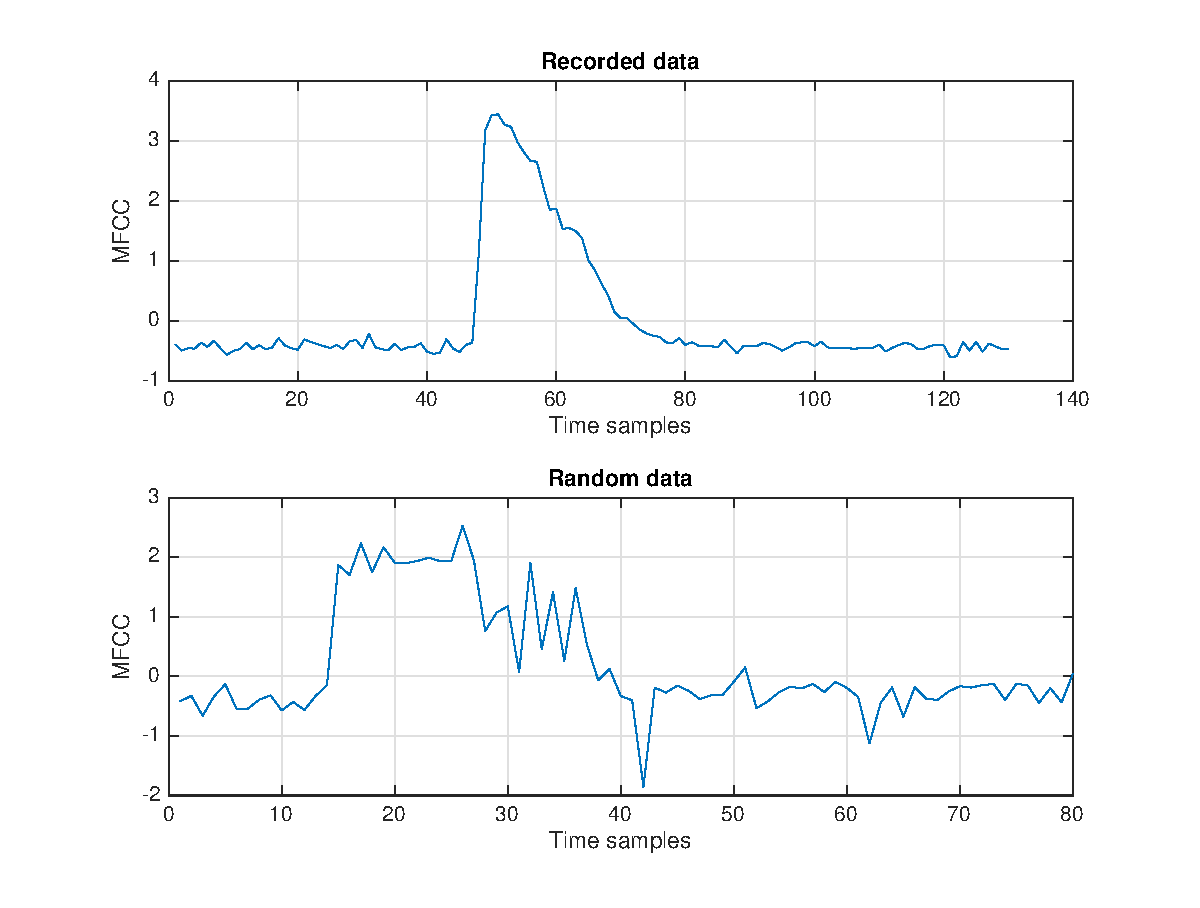
\includegraphics[width=0.65\textwidth]{figures/example}
\end{center}}
  \only<2>{
  \begin{itemize}
 \item word \textit{I} and 2nd MFCC coefficient
 \end{itemize}
\vspace{0mm}
\begin{center}
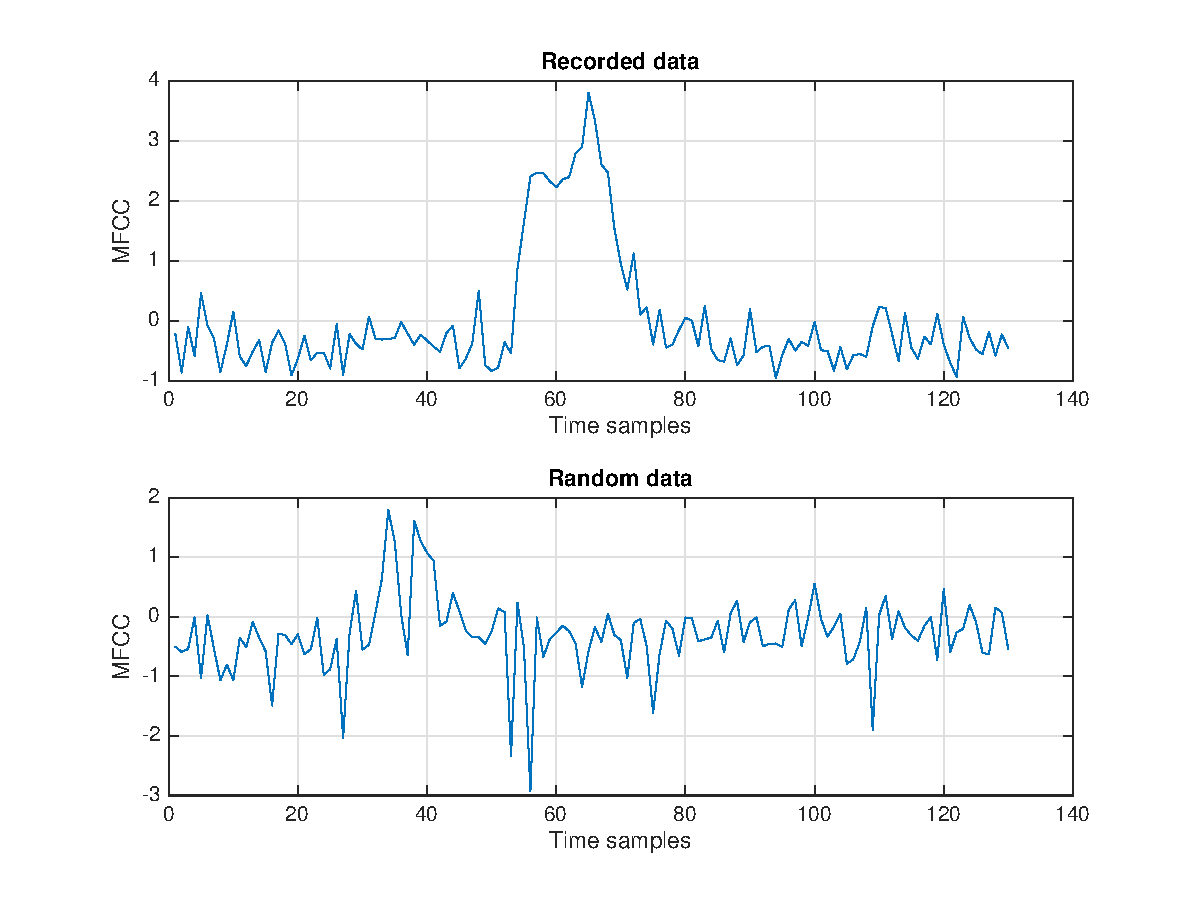
\includegraphics[width=0.65\textwidth]{figures/example2}
\end{center}}
 \end{frame}
 

 
%  \subsection{Varying Time Delay}
% %--------------------------------------------------------------------------------------------------
%% New frame
%%--------------------------------------------------------------------------------------------------
%\begin{frame}{\insertsection}{\insertsubsection}   
% 
%\headline{Varying Time Delay}
%\medskip
%\begin{itemize}
%	\uncover<2->{
%	\item  Dead-time sensitivity of MPC}
%	\uncover<3->{
%	\item  Possible Problem: Prediction horizone of MPC}
%	\uncover<4->{
%	\item MPC quality degrades if error between used model and real time delay increases}
%\end{itemize}
%
%\uncover<5->{
%\begin{block} \centering
%	Varying time delay results in the need of a \headline{robust} controller. Several possible solutions mentioned in papers...
%\end{block}
%}
 
% \end{frame}
 
 

 


 
\againframe<2>{contentframe}   % repeat the table of contents
%--------------------------------------------------------------------------------------------------
% Präsentation ICC-System:
%		Stand der Dinge in Sachen Rückkopplungskompensation und Ausblick
%
%--------------------------------------------------------------------------------------------------


\section{Results}

%~~~~~~~~~~~~~~~~~~~~~~~~~~~~~~~~~~~~~~~~~~~~~~~~~~~~~~~~~~~~~~~~~~~~~~~~~~~~~~~~~~~~~~~~~~~~~~~~~~
% New subsection
%~~~~~~~~~~~~~~~~~~~~~~~~~~~~~~~~~~~~~~~~~~~~~~~~~~~~~~~~~~~~~~~~~~~~~~~~~~~~~~~~~~~~~~~~~~~~~~~~~~
\subsection{System Performance}

%--------------------------------------------------------------------------------------------------
% New frame
%--------------------------------------------------------------------------------------------------
\begin{frame}{\insertsection}{\insertsubsection}   
 
\headline{Classification Errors}
\begin{itemize}
   \uncover<1->{
 \item Average Classification Error: 1.2 \%(validation) and 4.9 \% (overall) }
 \uncover<2->{
 \item Most commonly missclassified: \textit{hand} with 16.6 \% and  30 \%}
 \end{itemize}

 \end{frame}
 
 \begin{frame}{\insertsection}{\insertsubsection}   
 \vspace{-2mm}
 \only<1>{
C = 
$$
 \begin{pmatrix}
46	& 0 &	0 &	0	&0	&0	&0&	0&	0&14	&0&0	&0&	0 \\
0	&57	&0	&0	&3	&0&	0	&0	&0&	0	&0&	0	&0&	0\\
0	&0&	60&	0	&0	&0	&0	&0&	0&	0&	0&	0	&0&	0\\
0	&0&	0&	60	&0&	0	&0	&0	&0	&0	&0&	0	&0&	0\\
0	&0	&0&	0	&60	&0&	0&	0	&0	&0&	0&	0&	0	&0\\
0	&0&	0	&0	&0&	60	&0&	0&	0&	0&	0	&0	&0&	0\\
0	&0&0&	0&	0	&0	&60	&0&	0&	0&	0&	0	&0	&0\\
0	&0&	0	&0	&0	&0	&0&	60&	0&	0&	0&	0&	0&	0\\
0&	0&	0&	0&	0&	0	&0	&0&	57	&0	&1&	0	&0&	2\\
0	&0&	0	&0&	0	&0	&0	&0	&0	&60	&0	&0&	0	&0\\
0	&0&	7&	0	&0	&11&	0	&0	&0	&0&	42	&0	&0	&0\\
0	&0	&0&	0&	0	&0	&0&	0&	0	&0	&0&	60&	0&	0\\
0&	0	&0&	0	&1	&0&	0&	0&	0	&0	&0&	0	&57&	2\\
0	&0	&0&	0&	0&	0	&0	&0&	0&	0	&0	&0&	0&	60\\
 \end{pmatrix}
 $$}
 \only<2>{
 \movie[externalviewer]{Lars: recognition}{lars_recognition-01.wav}\\
  \movie[externalviewer]{Martin: recognition}{martin_recognition-01.wav}\\
\movie[externalviewer]{Natalie: recognition}{natalie_recognition-11.wav}}
 
  \end{frame}
  
  \subsection{Conclusion}

%--------------------------------------------------------------------------------------------------
% New frame
%--------------------------------------------------------------------------------------------------
\begin{frame}{\insertsection}{\insertsubsection}   
 
\headline{Take aways}
\medskip
\begin{itemize}
\uncover<1->{
\item If data is rare, use smaller k in k-fold approach}
\uncover<2->{
\item Good training data is important}
\uncover<3->{
\item Collect more training data (remember trade-off)\\
but: then be aware of overfitting!}
\end{itemize}
\uncover<4->{
\headline{The system}}
\begin{itemize}
\uncover<4->{
\item Satisfying overall recognition rate}
\uncover<5->{
\item Problems with the words \textit{hand} and \textit{recognition}}
\uncover<6->{
\item less problems with \textit{affect} and \textit{effect} or short words }
\end{itemize}







 \end{frame}
 
 \subsection{Live Demonstration}
 %--------------------------------------------------------------------------------------------------
% New frame
%--------------------------------------------------------------------------------------------------
\begin{frame}{\insertsection}{\insertsubsection}   
\headline{...}

 
 \end{frame}
 



%~~~~~~~~~~~~~~~~~~~~~~~~~~~~~~~~~~~~~~~~~~~~~~~~~~~~~~~~~~~~~~~~~~~~~~~~~~~~~~~~~~~~~~~~~~~~~~~~~~
% New subsection
%~~~~~~~~~~~~~~~~~~~~~~~~~~~~~~~~~~~~~~~~~~~~~~~~~~~~~~~~~~~~~~~~~~~~~~~~~~~~~~~~~~~~~~~~~~~~~~~~~~


%--------------------------------------------------------------------------------------------------
% End of document
%--------------------------------------------------------------------------------------------------
\end{document}
